\section{Results}
\label{sec:results}
This section presents an evaluation of our results and a discussion of the model's performance. We begin with a visual comparison between an estimated and ground-truth pose, followed by a detailed analysis of the model's performance on the test set. Finally, we examine the resulting trajectories from our localization pipeline.

\subsection{Visual Comparison of Estimated and Ground Truth Pose}
Figure \ref{fig:pose-comparison} illustrates a visual comparison between the estimated pose and the corresponding ground-truth from the test set, shown from four perspectives rotated at 0°, 90°, 180° and 270° angles. Overall, the estimated pose captures the global body posture of the target well. In particular, the global orientation of the skeleton and the left-leg joint positions align closely with the ground-truth. However, discrepancies are visible in the right lower leg, which appears shifted further back relative to the ground-truth. Furthermore, the estimated upper body exhibits a slightly stronger forward lean than the reference.

\begin{figure}[htbp]
    \centering
    \includegraphics[width=0.8\columnwidth]{img/pose_comparison.pdf}
    \caption{Comparison of a single estimated 3D pose (red) to its corresponding ground-truth pose (blue) from four different perspectives.}
    \Description{}
    \label{fig:pose-comparison}
\end{figure}

\subsection{Metrics}
Our recorded metrics for the testset mirror the comparison quite well. Figure \ref{fig:mjpe} shows the Mean Joint Position Error (MJPE) for all items from the testset. The hip was the easiest joint to estimate with about 2~cm mean error. This is because the hip moves the least in space and wrong estimations do not lead to a big error. On the other hand the most outer joints, the wrist and ankle, which move the most in space, performed the worst, with a median of about 6.5~cm and 7.5~cm. 

Secondly, there are quite some outliers with big errors up to 30~cm. This can represent an entirely different pose. These outliers occur for two reasons. Either the subject has just stepped on the floor and there is no history information available, which gives the model not enough information to estimate an accurate pose or the subject performs an unforseen action, for example by rapidly changing the directions or moving their body unnaturally. 

% Is there really a mismatch? The right angle and knee seem to perform better than the left side. Maybe just variance in data?
% More ideas to mention:
% - Why are the elbow and wrist estimations better than the angle estimations? (ankle is closest to floor and should be the best then?)
Thirdly, there is a tiny mismatch between the left and right side of the joints. By looking into the predicted poses from MediaPipe we found that the predicted height of the joints has different statistics. This is most likely due to our data collection setup where we recorded from a 45° angle leading to one side of the body being covered more by the rest of the body leading to small occlusion effects. This leads to a higher variance of the predictions from MediaPipe and a higher error and variance in the prediction errors which are compared to the predictions from MediaPipe. 

\begin{figure}[htbp]
    \centering
    \includegraphics[width=\columnwidth]{img/mjpe_boxplot.pdf}
    \caption{Mean Joint Position Error Boxplot for each joint on the testset with $n=21898$ samples. The box is the Interquartile Range (IQR) and the Whiskers extend the box by $1.5\times$ IQR. Left and Right are abbreviated to 'L.' and 'R.'}
    \Description{}
    \label{fig:mjpe}
\end{figure}

%Definition of Box Components: The caption (not provided here, but essential in the paper) must define what the box and whiskers represent. Typically:Center line = Median.Box = Interquartile Range (IQR).Whiskers = 1.5 $\times$ IQR or specific percentiles (e.g., 5th/95th).Sample Size ($n$): There is no indication of how many frames or sequences were used to generate this data. Adding "$n = \text{number of samples}$" in the caption or text is necessary for reproducibility.
Furthermore the figure explains the big difference for the results of the Percentage Correct Key points (PCK) between a 5~cm and 10~cm threshold on the ankles.
As the Interquartile range for the MJPE of the feet ankles lay just above 5~cm the PCK for this threshold is $37\%$ where for 10~cm it is $72\%$.
The mean PCK for 5~cm is $61\%$ and for 10~cm it is $87\%$.
\todo{should we Maybe the val\_loss graph or sth would be nice}
The other values and the training graph can be found in the annex.



% - Predicted pose compared to true pose image
% - Training metrics (boxplot and mention pck) explain tha numbers


% - Estimated position (House of Kalmann)
\subsection{Localization and Kalman-Filter Effect}
In \ref{subsec:localization}, we introduced our approach for extracting information about the person's current global position from the SensFloor activation signals. The left side of Figure \ref{fig:kalman-filter-effect} shows the raw clustering position trajectory we recorded during a test walk. The illustrated trajectory is highly erratic. This instability is caused by two main factors. First, the algorithm creates jumps in the estimated position as the mean shifts abruptly whenever a foot makes or breaks contact with the floor. Second, the SensFloor fields produce significant background noise, even in areas where no activity takes place. While increasing the noise signal threshold suppresses some of the noise, it is not a universal solution, as signal intensity of people moving on the floor varies depending on the person's footwear. 

However, applying the Kalman filter largely reduces these issues, as illustrated on the right side of Figure \ref{fig:kalman-filter-effect}. By smoothing out the abrupt transitions and mitigating the impact of outliers, the filter produces a smooth and, according to our empirical evaluation, accurate trajectory.

\todo{set the arrows to a fixed size, so it's not confusing}
\begin{figure}[htbp]
    \centering
    \includegraphics[width=\columnwidth]{img/kalman-filter-effect.pdf}
    \caption{Comparison of raw (left) and filtered (right) localization trajectories. The arrows indicate the direction of the movement.}
    \Description{}
    \label{fig:kalman-filter-effect}
\end{figure}
% - Inference works



% - evaluation
    % - Mediapipe inconsistency
    % - Only male subjects for training
    % - No groundtruth for kalman filter
    % - testset split? No evaluation that our test and trianing set have a similar distribution
    % - Model learned to Look down
    % - Only small sequences of walking possible due to the small floor (and missing API endpoint with good estimations probably)